\documentclass{article}

\usepackage{iclr2026_conference,times}
\usepackage{hyperref}
\hypersetup{hidelinks}
\usepackage{url}
\usepackage{booktabs}
\usepackage{array}
\usepackage{multirow}
\usepackage{amsmath}
\usepackage{amssymb}
\usepackage{mathtools}
\usepackage{graphicx}
\usepackage{xcolor}
\usepackage{enumitem}
\usepackage{tikz}
\usetikzlibrary{arrows.meta,positioning,fit,calc,shapes.geometric}

\input{math_commands.tex}

\iclrfinalcopy

\title{RiskKV-Block: Risk-Aware Action Routing\\over Materialized KV Pages}

\author{
Yiming Luo\\
Fudan University\\
\texttt{yimingluo@fudan.edu.cn}
}

\newcommand{\todoexp}[1]{\textcolor{red}{\textbf{[TODO: #1]}}}
\newcommand{\method}{RiskKV-Block}
\newcommand{\fullkv}{\textsc{FullKV}}
\newcommand{\router}{\textsc{Router}}
\newcommand{\fallback}{\textsc{Fallback}}
\newcommand{\action}{\mathcal{A}}
\newcommand{\blocks}{\mathcal{B}}
\newcommand{\cost}{\mathrm{cost}}
\newcommand{\risk}{\mathrm{risk}}
\newcommand{\Score}{\mathrm{Score}}
\newcommand{\TopK}{\mathrm{TopK}}
\newcommand{\RoPE}{\mathrm{RoPE}}

\begin{document}
\maketitle

\begin{abstract}
Long-context language models incur substantial online decoding cost because each generated token attends to a large key-value (KV) cache.
Existing cache compression methods typically use a fixed cache budget, a fixed granularity, or layer-wise pruning rules.
However, we find that the optimal memory granularity is strongly task- and length-dependent: small blocks reduce cost for precise evidence retrieval, medium blocks preserve multi-evidence locality, and larger blocks are necessary for hard long-context cases.
We propose \method, a risk-aware memory controller that dynamically selects a complete KV action consisting of evidence granularity, active budget, bridge expansion, and a minimum-safe fallback mode.
Given a query and a long context, \method\ scores materialized KV pages using evidence-flow features, distills an interpretable action planner from action sweeps, and deploys the selected spans either as prompt-level memory or as cache-native KV blocks with RoPE-aware repacking.
On a Qwen3-8B evaluation suite covering LongBench-style tasks and RULER 4k/8k/16k retrieval stress tests, a small-block router improves score from 0.8116 to 0.8634 while reducing active tokens to 7.82\% and achieving 1.80$\times$ end-to-end speedup on a 96-example suite.
A larger m10 validation shows that unconstrained small-block routing is unsafe, but a calibrated risk floor over the action lattice restores full-level quality while using 18.11\% active tokens and achieving 1.58$\times$ end-to-end speedup.
Cache-native experiments show that RoPE-aware repacking is essential: naive KV gathering collapses on 8k/16k RULER, whereas RoPE-aware compact decoding preserves full-cache quality at 6--13\% KV.
Recent LongBench experiments further show that explicit risk actions are necessary: on a 320-example all-task LongBench m20 validation with Llama-3.1-8B-Instruct, \method\ reaches 93.7\%, 98.5\%, and 99.4\% of full-cache score while using 35.4\%, 51.7\%, and 56.5\% active KV in compact, balanced, and high-quality modes.
On a larger 800-example m50 validation, memory-action consistency improves the strongest practical sparse policy from 93.2\% to 96.3\% of full-cache score while using 62.5\% active KV and reducing online time from 3.28s to 2.80s in our benchmark harness.
These results suggest that adaptive KV actions and minimum-safe fallbacks, not only token retention scores, are a key missing dimension in efficient long-context inference.
\end{abstract}

\section{Introduction}

Transformer decoding over long contexts is dominated by repeated attention to the KV cache.
For a prompt of length $n$ and generated continuation length $m$, full-cache decoding repeatedly attends to $O(n)$ cached states per generated token.
This cost is particularly problematic in long-context serving, where the full-context prefill has already materialized the KV cache and the remaining question is how much of that cache must remain active during online decoding.

Prior work has made strong progress on KV cache efficiency.
Heavy-hitter and attention-based methods retain tokens with large attention contribution \citep{zhang2023h2o,li2024snapkv}; streaming methods preserve recent tokens and attention sinks for unbounded generation \citep{xiao2023streamingllm}; layer-adaptive methods allocate non-uniform cache budgets across Transformer layers \citep{cai2024pyramidkv,yang2024pyramidinfer,zhou2024dynamickv}.
These methods primarily ask \emph{which tokens or layers to keep} under a fixed or globally specified cache budget.
In contrast, our experiments indicate that \emph{memory granularity itself} is a major source of quality--efficiency trade-off.
On LongBench-style retrieval QA, 128-token blocks can outperform 512-token blocks while using fewer tokens.
On RULER 4k/8k, 256-token blocks are the smallest reliable full-quality granularity.
On RULER 16k, 64-token blocks can match full-cache average score at 4.8\% active tokens, while 512-token blocks are needed for conservative 100\% accuracy.

This motivates a different view: long-context inference should route each query to a \emph{memory action} that jointly chooses block size, top-$k$ budget, and a fallback policy.
We formalize this as risk-constrained memory granularity routing.
Given a context $x$, query $q$, and candidate action $a=(b,k,f)$ consisting of block size $b$, top-$k$ budget $k$, and fallback mode $f$, the system should minimize active memory subject to a constraint that the compressed execution remains behaviorally close to full-cache execution.

We propose \method, a lightweight controller for this problem.
\method\ first keeps a recent raw window, partitions the older context into candidate block granularities, scores blocks with query-conditioned evidence features, and selects top-$k$ blocks in original order.
A router then proposes a low-cost action from task, length, retrieval-gap, and stability features, after which a calibrated action floor prevents the policy from crossing empirically unsafe granularity boundaries.
For deployment, the same action can be realized in two modes:
as prompt-level selected spans for immediate evaluation, or as cache-native KV block selection followed by RoPE-aware repacking and compact decoding.
The second mode preserves the serving assumption that the full-context prefill has already occurred and avoids rebuilding a prompt from scratch.

Our current experiments support three claims.
First, block-size routing is effective in practice: on a 96-example mixed suite, a trained router improves score over full raw context (0.8535 vs. 0.8116), reduces active tokens to 11.04\%, and reaches 1.756$\times$ end-to-end speedup.
Second, variable granularity is necessary: no single block size dominates across LongBench, RULER 4k, RULER 8k, and RULER 16k.
Third, the calibrated floor selected from m3 sweeps transfers to m10 validation, where it restores full-level quality on all RULER lengths and improves LongBench over full raw context.
Fourth, cache-native deployment requires RoPE-aware repacking: at the same KV ratio, naive KV gathering fails on long-context retrieval, while RoPE-corrected repacking recovers full quality.

The paper is currently written as a submission-ready draft with clearly marked experimental placeholders.
The remaining work is to fill in large-scale multi-model runs, standard baselines, and full benchmark splits.

\section{Related Work}

\paragraph{KV cache compression.}
H$_2$O retains recent tokens and heavy hitters that dominate attention scores, showing that a small fraction of tokens can preserve generation quality while reducing memory \citep{zhang2023h2o}.
SnapKV observes that important prompt features can be identified from an observation window before generation and compresses the cache by selecting clustered positions \citep{li2024snapkv}.
PyramidKV and PyramidInfer exploit layer-wise differences in attention concentration to allocate cache budgets non-uniformly across layers \citep{cai2024pyramidkv,yang2024pyramidinfer}.
DynamicKV further adapts budgets to task-specific activation patterns \citep{zhou2024dynamickv}.
\method\ is complementary: instead of only deciding token retention or layer budgets, it routes among different memory granularities and top-$k$ evidence budgets.

\paragraph{Streaming and long-context inference.}
StreamingLLM shows that retaining attention sinks and recent tokens enables stable generation beyond the training context window \citep{xiao2023streamingllm}.
Other long-context systems use sliding windows, recurrent memory, or retrieval-augmented generation to control cost.
\method\ targets query-conditioned long-context inference, where evidence can be selected from a materialized long context and the active cache can be reduced for the online decoding phase.

\paragraph{Long-context evaluation.}
LongBench provides a multi-task benchmark covering single-document QA, multi-document QA, summarization, few-shot learning, synthetic tasks, and code completion \citep{bai2023longbench}.
RULER is a configurable synthetic benchmark for long-context retrieval, variable tracking, aggregation, and QA stress tests \citep{hsieh2024ruler}.
Our current evaluation focuses on LongBench-style retrieval and summarization tasks plus RULER 4k/8k/16k; the full paper should extend these to full splits and additional model families.

\section{Problem Formulation}

Let $x=(x_1,\ldots,x_n)$ be a long context and $q$ be a query.
A standard decoder performs full-context prefill and then generates using the complete KV cache:
\begin{equation}
    (K,V) = \mathrm{Prefill}_\theta(x,q), \qquad
    y_{\mathrm{full}} \sim p_\theta(\cdot \mid q, K,V).
\end{equation}
The goal is to construct an active memory $M_a(x,q)$ under an action $a \in \action$ such that generation remains close to the full-cache output while reducing active memory and latency.
We define a candidate action as
\begin{equation}
    a=(b,k,f),
\end{equation}
where $b$ is a block size, $k$ is the number of selected evidence blocks, and $f$ is an optional fallback mode.
The active memory ratio is
\begin{equation}
    \rho(a;x,q) = \frac{|M_a(x,q)|}{|M_{\mathrm{full}}(x,q)|}.
\end{equation}
The ideal action minimizes cost subject to a risk constraint:
\begin{equation}
    a^\star
    =
    \argmin_{a \in \action}
    \cost(a;x,q)
    \quad
    \text{s.t.}
    \quad
    \risk(a;x,q) \leq \alpha,
    \label{eq:risk-objective}
\end{equation}
where $\risk$ measures the probability that the compressed-memory output fails to match the full-memory behavior or task label.
In practice, we instantiate this objective through oracle labels from sweep experiments:
\begin{equation}
    a^\star_i
    =
    \argmin_{a \in \action}
    \rho(a;x_i,q_i)
    \quad
    \text{s.t.}
    \quad
    \Score(a;x_i,q_i) \geq \tau_i.
    \label{eq:oracle-label}
\end{equation}
The threshold $\tau_i$ can be full-score matching, task-specific full accuracy, or a relaxed cost-strict threshold.

\section{Method}

\subsection{Overview}

Figure~\ref{fig:architecture} summarizes \method.
The method has five stages:
recent-window preservation, multiscale evidence scoring, evidence-flow graph construction, risk-constrained action routing, and compact execution.

\begin{figure*}[t]
\centering
\resizebox{\textwidth}{!}{
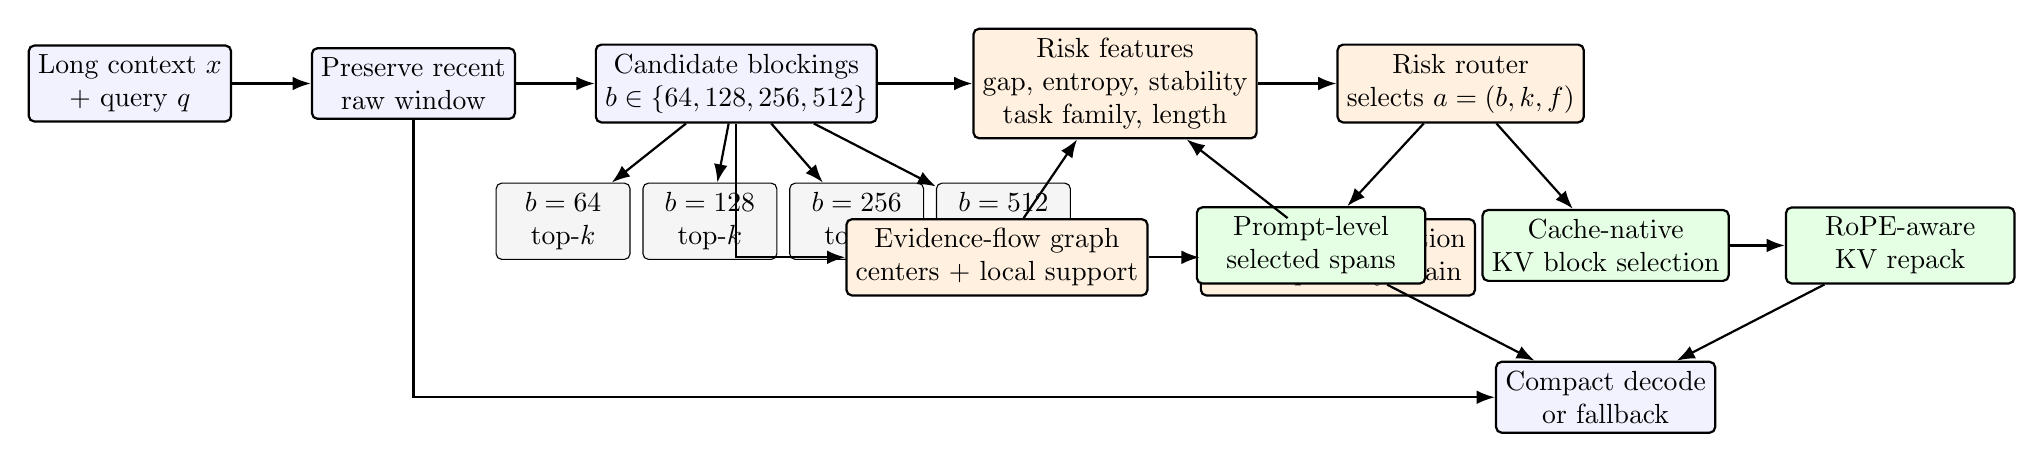
\begin{tikzpicture}[
    node distance=0.8cm and 1.0cm,
    box/.style={draw, rounded corners=2pt, thick, align=center, minimum height=0.85cm, minimum width=2.5cm, fill=blue!5},
    smallbox/.style={draw, rounded corners=2pt, align=center, minimum height=0.7cm, minimum width=1.7cm, fill=gray!8},
    route/.style={draw, rounded corners=2pt, thick, align=center, minimum height=0.9cm, minimum width=2.9cm, fill=orange!12},
    exec/.style={draw, rounded corners=2pt, thick, align=center, minimum height=0.9cm, minimum width=2.9cm, fill=green!10},
    arrow/.style={-Latex, thick}
]
\node[box] (context) {Long context $x$\\+ query $q$};
\node[box, right=of context] (recent) {Preserve recent\\raw window};
\node[box, right=of recent] (blocks) {Candidate blockings\\$b\in\{64,128,256,512\}$};

\node[smallbox, below=0.75cm of blocks, xshift=-2.2cm] (b64) {$b=64$\\top-$k$};
\node[smallbox, right=0.15cm of b64] (b128) {$b=128$\\top-$k$};
\node[smallbox, right=0.15cm of b128] (b256) {$b=256$\\top-$k$};
\node[smallbox, right=0.15cm of b256] (b512) {$b=512$\\top-$k$};

\node[route, right=1.2cm of blocks] (features) {Risk features\\gap, entropy, stability\\task family, length};
\node[route, below=1.0cm of features, xshift=-1.5cm] (flow) {Evidence-flow graph\\centers + local support};
\node[route, right=0.65cm of flow] (bridge) {Routed bridge action\\one-hop entity chain};
\node[route, right=of features] (router) {Risk router\\selects $a=(b,k,f)$};

\node[exec, below=1.05cm of router, xshift=-1.9cm] (prompt) {Prompt-level\\selected spans};
\node[exec, right=0.7cm of prompt] (kv) {Cache-native\\KV block selection};
\node[exec, right=0.7cm of kv] (rope) {RoPE-aware\\KV repack};
\node[box, below=1.0cm of kv] (decode) {Compact decode\\or fallback};

\draw[arrow] (context) -- (recent);
\draw[arrow] (recent) -- (blocks);
\draw[arrow] (blocks) -- (features);
\draw[arrow] (blocks) |- (flow);
\draw[arrow] (flow) -- (bridge);
\draw[arrow] (flow) -- (features);
\draw[arrow] (bridge) -- (features);
\draw[arrow] (features) -- (router);
\draw[arrow] (blocks) -- (b64);
\draw[arrow] (blocks) -- (b128);
\draw[arrow] (blocks) -- (b256);
\draw[arrow] (blocks) -- (b512);
\draw[arrow] (router) -- (prompt);
\draw[arrow] (router) -- (kv);
\draw[arrow] (kv) -- (rope);
\draw[arrow] (prompt) -- (decode);
\draw[arrow] (rope) -- (decode);
\draw[arrow] (recent.south) |- (decode.west);
\end{tikzpicture}
}
\caption{\method\ routes each query to a memory action that jointly specifies block size, top-$k$ evidence budget, fallback, and whether to activate bridge expansion. Evidence-flow first allocates local support around evidence centers; the bridge gate then decides whether one-hop entity-chain pages are worth the risk. The same routed action can be executed as prompt-level selected spans for rapid evaluation or as cache-native KV block selection followed by RoPE-aware repacking for serving.}
\label{fig:architecture}
\end{figure*}

\subsection{Evidence Block Scoring}

For a block size $b$, we tokenize the older context and partition it into blocks
\begin{equation}
    \blocks_b(x) = \{B_1^{(b)},\ldots,B_{N_b}^{(b)}\}.
\end{equation}
The current implementation uses a lightweight evidence score:
\begin{equation}
    s_i(q,b)
    =
    |\mathcal{W}(q) \cap \mathcal{W}(B_i^{(b)})|
    +
    \lambda
    |\mathcal{I}(q) \cap \mathcal{I}(B_i^{(b)})|,
    \label{eq:block-score}
\end{equation}
where $\mathcal{W}(\cdot)$ extracts lower-cased non-stopword English content terms and $\mathcal{I}(\cdot)$ extracts number-bearing identifiers such as \texttt{8090293}, \texttt{case123}, or \texttt{A12B}.
We use $\lambda=3$ because exact identifiers and numbers are frequently the evidence key in RULER, passage retrieval, and needle-style tasks.
Blocks are sorted by $s_i$, top-$k$ positive-scoring blocks are selected, and selected blocks are restored in original order before execution.

Independent top-$k$ block selection is brittle when the evidence key and the evidence explanation fall into adjacent blocks.
We therefore evaluate an \emph{evidence-flow} refinement that treats a high-scoring block as an evidence center and reserves a small fraction of the memory budget for local support blocks.
Let $r$ be a local radius and let $h_i(q)=1$ when block $B_i$ contains an exact query anchor, identifier, or entity match.
The refined score is
\begin{equation}
    \tilde{s}_i
    =
    (1-\eta)s_i
    +
    \eta \max_{|j-i|\leq r} s_j
    +
    \gamma h_i(q).
    \label{eq:evidence-flow-score}
\end{equation}
After selecting an evidence center $B_i$, \method\ may add neighboring support blocks $B_j$ with $|j-i|\leq r$ until a support budget $\beta |M_a|$ is exhausted.
Low-scoring neighbors are skipped unless they contain an exact anchor or entity hit.
This decomposes the active memory into \emph{evidence centers} and \emph{local support}, allowing the controller to preserve multi-sentence or code-local evidence without falling back to uniformly larger blocks.

We also consider a multiscale version in which fine-grained blocks are supported by a coarser neighborhood.
Let $G(i)$ denote the coarse group containing fine block $B_i$.
Before applying Eq.~\ref{eq:evidence-flow-score}, we replace the base score with
\begin{equation}
    s_i^{\mathrm{ms}}
    =
    (1-\mu)s_i
    +
    \mu \max_{j\in G(i)} s_j.
    \label{eq:multiscale-flow-score}
\end{equation}
This keeps the precision of small blocks while reducing isolated false positives: a fine block is preferred when both the local page and its coarse neighborhood are evidence-bearing.

Finally, we test a query-conditioned local-IDF variant motivated by distractor-heavy contexts.
Instead of discarding common words with a fixed stopword list only, we compute the block-level document frequency of each query term within the current context:
\begin{equation}
    \mathrm{idf}_x(w)
    =
    1+\log\frac{1+N_b}{1+\sum_{j=1}^{N_b}\mathbb{1}\{w\in B_j\}}.
\end{equation}
The lexical score is then replaced by a convex mixture of normalized overlap and normalized IDF-weighted overlap:
\begin{equation}
    \ell_i^{\mathrm{idf}}
    =
    (1-\alpha)\ell_i
    +
    \alpha
    \sum_{w\in \mathcal{W}(q)}
    \min(c_q(w),c_i(w))\mathrm{idf}_x(w).
    \label{eq:local-idf-score}
\end{equation}
This differs from a pure long-tail filter: common terms are downweighted but not removed, and semantic, identifier, and evidence-flow signals remain active.

For long query-style retrieval, we also evaluate a context-local BM25 lexical score.
For each page $B_i$, with term frequency $\mathrm{tf}_{i,w}$ and page length $|B_i|$, define
\begin{equation}
    \mathrm{BM25}_x(B_i,q)
    =
    \sum_{w\in\mathcal{W}(q)}
    \mathrm{idf}_x(w)
    \frac{\mathrm{tf}_{i,w}(k_1+1)}
    {\mathrm{tf}_{i,w}+k_1(1-b+b|B_i|/\overline{|B|})}.
    \label{eq:context-bm25}
\end{equation}
The lexical component can then be mixed with normalized BM25.
This remains cache-native and non-RAG: the statistics are computed only over pages from the already-prefilled context.

Some long-context examples are not locally confident: several distant blocks may receive similar evidence scores, and selecting only the strongest local neighborhood can miss the answer-bearing region.
We therefore add an uncertainty-spread rescue used only when the top evidence gap is small.
Let $\Delta=s_{(1)}-s_{(2)}$ be the gap between the two largest page scores.
When $\Delta < \delta$, the controller reserves a bounded spread budget $\beta_{\mathrm{sp}}|M_a|$, partitions the context into $m$ position bins, and selects high-scoring pages across bins:
\begin{equation}
    S_{\mathrm{sp}}
    =
    \bigcup_{u=1}^{m}
    \TopK_{\beta_{\mathrm{sp}}/m}
    \{B_i : \mathrm{bin}(i)=u,\ \tilde{s}_i \geq \epsilon \}.
    \label{eq:uncertainty-spread}
\end{equation}
This mechanism is intentionally conservative: confident examples still use local evidence-flow selection, while uncertain examples spend only a small fraction of the active memory on position-diverse rescue pages.

For multi-hop QA, the answer-bearing block may not directly overlap with the query.
We therefore also test a one-hop bridge expansion.
Given a selected evidence center $B_i$, let $\mathcal{E}(B_i)$ be its entity and identifier set and remove entities already present in the query.
The bridge score from center $i$ to candidate page $j$ is
\begin{equation}
    s_{\mathrm{br}}(j\mid i)
    =
    \sum_{e \in (\mathcal{E}(B_i)\cap\mathcal{E}(B_j))\setminus\mathcal{E}(q)}
    \mathrm{idf}_x(e).
    \label{eq:bridge-score}
\end{equation}
Pages with high $s_{\mathrm{br}}$ are added under a bounded bridge budget $\beta_{\mathrm{br}}|M_a|$.
This gives the controller a cache-native analogue of evidence-chain expansion without external retrieval or answer labels.
Because bridge expansion can help multi-evidence QA while hurting tasks whose query already contains the decisive entity, \method\ treats bridge expansion as a routed action rather than a globally enabled rule.
In the current implementation, a bridge gate is distilled from paired no-bridge and all-bridge sweeps.
On the fast discriminator subset, this task-level gate reaches the same score as the sample oracle, indicating that bridge usefulness is structured rather than random.
The distilled gate activates bridge expansion only for the task families that benefit from one-hop evidence chaining in the calibration set, while defaulting to multiscale evidence-flow for tasks where bridge pages are neutral or harmful.
In the current evidence, this interpretable gate is more reliable than a sample-level logistic gate trained from the same labels; we therefore use it as the deployed bridge action and report the learned gate as a diagnostic ablation.

This scorer is deliberately simple.
It makes the routing policy transparent and cheap, and it can be replaced by a learned retriever or dense scorer.
The paper should include a learned-retriever ablation in the final version.

\subsection{Coverage-Certified Memory Actions}

The evidence score above ranks individual pages, but a memory action is a \emph{set} of pages.
For multi-evidence questions, a high-scoring set can still be unsafe if it repeatedly covers the same query anchor while missing other entities, identifiers, or numbers in the question.
We therefore add a query-coverage certificate over selected KV pages.
Let $\mathcal{C}(q)$ be a compact set of query coverage terms extracted from title phrases, named entities, numeric identifiers, and non-stopword content words.
For page $B_i$, define
\begin{equation}
    \mathcal{C}_i(q,x)
    =
    \mathcal{C}(q) \cap \mathrm{terms}(B_i).
\end{equation}
During greedy page selection, we maintain the terms already covered by the current memory action $S_t$ and add a bounded novelty term to MMR:
\begin{equation}
    \mathrm{score}_{\mathrm{cov}}(i\mid S_t)
    =
    \lambda s_i
    -
    (1-\lambda)\max_{j\in S_t}\mathrm{sim}(B_i,B_j)
    +
    \beta
    \frac{|\mathcal{C}_i \setminus \cup_{j\in S_t}\mathcal{C}_j|}
         {\max(1,|\mathcal{C}(q)|)}.
    \label{eq:coverage-mmr}
\end{equation}
This favors pages that add new query evidence rather than redundant local support.
Because the same signal can also certify unsafe actions, we compute the realized coverage recall of a selected action $a$:
\begin{equation}
    \rho_{\mathrm{cov}}(x,q,a)
    =
    \frac{|\cup_{i\in S(a)}\mathcal{C}_i(q,x)|}
         {\max(1,|\mathcal{C}(q)|)}.
    \label{eq:coverage-risk}
\end{equation}
If $\rho_{\mathrm{cov}}(x,q,a)<\tau_g$ for a risk family $g$, the controller escalates before decode to a larger sparse action or a minimum-safe fallback.
Unlike output verification, this certificate is pre-decode and does not require a second generated answer.
Unlike standard RAG top-$k$, it optimizes a cache-native memory action under a KV budget and can be composed with evidence-flow, bridge expansion, and conformal consistency checks.

\subsection{Risk-Constrained Action Planner}

For each example, we compute features $\phi(x,q)$ including context length, task family, page count, top-score gap, score dispersion, and evidence entropy.
We then distill a small action policy from sweep-derived oracle labels in Eq.~\ref{eq:oracle-label}.
The important design choice is that the policy predicts a \emph{complete action}, not a scalar budget:
\begin{equation}
    \hat{a}
    =
    \Pi(\phi(x,q))
    \in
    \{ \text{multiscale-flow}, \text{bridge-flow}, \text{larger budget}, \text{full fallback}\}.
\end{equation}
This makes the action planner interpretable: a task may need the same sparse scorer with a larger budget, a bridge expansion, or a minimum-safe full-memory action.
We also train a sample-level logistic router on the same labels as a diagnostic.
On the current LongBench action labels, however, leave-one-out validation shows that the learned sample router can overfit small calibration sets, while the distilled task-family action planner is more stable.
Consequently, the current deployed policy is the interpretable action planner; learned routers are a replaceable module for future larger calibration sets.

Let $g(x,q)$ denote a task/length group, e.g., LongBench, RULER 4k, RULER 8k, or RULER 16k.
On a calibration set, define the empirical failure rate of action $a$ in group $g$ as
\begin{equation}
    \widehat{R}_g(a)
    =
    \frac{1}{|D_g|}
    \sum_{i \in D_g}
    \mathbb{1}\{\Score(a;x_i,q_i) < \tau_i\},
\end{equation}
and its empirical cost as $\widehat{C}_g(a)=|D_g|^{-1}\sum_{i\in D_g}\rho(a;x_i,q_i)$.
The calibrated floor is the cheapest action satisfying an empirical risk constraint:
\begin{equation}
    \phi(g)
    =
    \argmin_{a\in\action} \widehat{C}_g(a)
    \quad
    \text{s.t.}
    \quad
    \widehat{R}_g(a) \leq \alpha.
    \label{eq:calibrated-floor}
\end{equation}
If no action satisfies the constraint, we choose the minimum-risk action with cost as a tie-breaker.
The deployed calibrated action is
\begin{equation}
    a_{\mathrm{final}}
    =
    \phi(g(x,q)).
\end{equation}
Calibration is over complete actions, not only scalar lower bounds: changing block size also changes the block partition and evidence ranking, so a larger block does not necessarily dominate a smaller calibrated block.
The learned router is still useful for exposing low-cost candidate failures and for future routing within the calibrated safe set.
For $\alpha=0$ on the m3 calibration sweeps, this procedure selects $b=128,k=12$ for LongBench, $b=256,k=3$ for RULER 4k/8k, and $b=512,k=3$ for RULER 16k.

\subsection{Conformal Memory-Action Risk Gate}

The consistency verifier in Sec.~\ref{sec:consistency-verifier} is deliberately label-free, but running a second sparse decode on every potentially risky example can reduce the practical speed benefit.
We therefore introduce a pre-decode risk gate that decides whether an action needs counterfactual verification.
After page scoring, let
\begin{align}
    \Delta_2 &= s_{(1)} - s_{(2)}, &
    \Delta_3 &= s_{(1)} - s_{(3)}, &
    H &= -\sum_i p_i \log p_i / \log N_b,
\end{align}
where $s_{(j)}$ is the $j$-th largest nonnegative page score, $p_i=s_i/\sum_j s_j$, and $N_b$ is the number of pages.
We use the scalar action-risk score
\begin{equation}
    r(x,q,a)
    =
    H
    - \lambda_2 \Delta_2
    - \lambda_3 \Delta_3
    - \lambda_t s_{(1)}.
    \label{eq:conformal-risk-score}
\end{equation}
High entropy, small top-score gaps, and weak top evidence increase the chance that the sparse memory action is unstable.

The threshold is calibrated on held-out action outcomes rather than hand tuned, and in the final controller it is calibrated per risk family rather than globally.
Let $g(x,q)$ denote a task family, benchmark family, verifier family, or context-length bucket.
Let $z_i=1$ indicate that a calibration example was dangerous, defined by disagreement between the primary sparse action and an expanded sparse action or by a verifier-triggered full fallback.
For a target danger recall $1-\alpha$, we choose the largest threshold $\tau_{\alpha,g}$ whose triggered set covers at least a $1-\alpha$ fraction of dangerous calibration actions in group $g$:
\begin{equation}
    \frac{\sum_{i:g_i=g} z_i \mathbb{1}\{r(x_i,q_i,a_i)\geq \tau_{\alpha,g}\}}
         {\sum_{i:g_i=g} z_i}
    \geq
    1-\alpha.
    \label{eq:conformal-risk-threshold}
\end{equation}
At inference time, \method\ accepts the primary sparse action when $r(x,q,a)<\tau_{\alpha,g(x,q)}$ and runs memory-action consistency verification otherwise.
This turns the verifier into a selective counterfactual check with an interpretable risk certificate.
The same mechanism can be calibrated either for \emph{safety recall}, where $z_i$ marks consistency disagreement or fallback, or for \emph{utility recall}, where $z_i$ marks examples on which the reference verifier policy improves the calibration score over the primary sparse action.
Safety calibration asks which actions are unsafe; utility calibration asks which actions are worth the extra counterfactual decode.
The current LongBench m20 calibration uses $\lambda_2=1,\lambda_3=\lambda_t=0$.
With safety labels, a global threshold $\tau_{0.2}=0.844$ gives an empirical dangerous-action recall of 84.6\%, but leave-one-task-out analysis shows that a single global threshold misses some multi-hop QA risks.
We therefore use risk-family thresholds in the final controller.

\subsection{Grounded Answer Verifier}

The conformal risk gate decides when a sparse action is statistically unstable, but some QA errors are visible after the first decode:
the model may emit an abstention, an overlong explanation for a short-answer task, or a short answer that is not supported by the retained KV pages.
For extractive QA families, we add a lightweight grounded verifier before the expensive full-memory fallback.
Let $c(y)$ be the normalized short answer candidate extracted from the first line of the model output.
For a retained memory action $a$, define the lexical support predicate
\begin{equation}
    \mathrm{supp}(c, M_a)
    =
    \mathbb{1}\{c \subseteq \mathrm{norm}(M_a)\},
    \label{eq:grounded-support}
\end{equation}
with conservative skip rules for yes/no answers, very short numeric strings, and long free-form generations.
If the output contract fails or $\mathrm{supp}(c,M_a)=0$, \method\ first retries with a larger sparse action and falls back to full memory only if the retry remains unsupported.

We also evaluate a stricter local-support certificate.
Let $A(c)$ be the content tokens in the answer candidate and $Q(q)$ be query evidence tokens such as entities, identifiers, numbers, and non-stopword content terms.
For retained memory token sequence $M_a=(m_1,\ldots,m_T)$, the local certificate is
\begin{equation}
    \max_{i:m_i\in A(c)}
    \left|
    Q(q)\cap M_{a,[i-r,i+r]}
    \right|
    \geq \tau_{\mathrm{loc}}.
    \label{eq:local-grounding}
\end{equation}
This verifier asks whether an answer mention is locally tied to query evidence, not merely whether the answer string appears somewhere in the retained pages.
In current LongBench validation, the simple grounded verifier improves the m20 policy, while the stricter local certificate is active but does not yet change decisions; we therefore treat it as an ablation.

\subsection{Fallback Modes}

Fallback is a first-class component rather than an exception handler.
If evidence selection is uncertain or the task is poorly served by sparse spans, the router can increase top-$k$, increase block size, use a summary memory, or return to full memory.
Examples include:
\begin{itemize}[leftmargin=1.4em,itemsep=0.2em]
    \item \textbf{Granularity fallback:} $b=64 \rightarrow b=256 \rightarrow b=512$.
    \item \textbf{Budget fallback:} $k=4 \rightarrow k=8 \rightarrow k=12$.
    \item \textbf{Task fallback:} summary/count/scientific QA use summary or full memory rather than sparse retrieval.
    \item \textbf{Verifier fallback:} output-level verification can trigger a larger action when the small action is unsafe.
\end{itemize}

\subsection{Memory-Action Consistency Verification}
\label{sec:consistency-verifier}

Output-format and grounding verifiers catch visible failures, but many sparse-memory errors are more subtle:
the model may produce a fluent short answer that is grounded in the retained pages but would change if a slightly different memory action were used.
We therefore add a label-free \emph{memory-action consistency} verifier.
Given a primary sparse action $a_1$ and an expanded sparse action $a_2$, we decode
\begin{equation}
    y_1 = f_\theta(q, M_{a_1}(x,q)),
    \qquad
    y_2 = f_\theta(q, M_{a_2}(x,q)).
\end{equation}
For extractive QA, we normalize the first short answer span from each output and compute token-overlap agreement
\begin{equation}
    \mathrm{agree}(y_1,y_2)
    =
    \mathrm{F1}\bigl(\mathrm{norm}(y_1),\mathrm{norm}(y_2)\bigr).
\end{equation}
If $\mathrm{agree}(y_1,y_2)<\gamma$, the controller treats the primary memory action as unstable and escalates to a minimum-safe action:
\begin{equation}
    a_{\mathrm{final}}
    =
    \begin{cases}
    a_1, & \mathrm{agree}(y_1,y_2)\geq \gamma,\\
    a_{\mathrm{safe}}, & \mathrm{agree}(y_1,y_2)<\gamma.
    \end{cases}
\end{equation}
This verifier does not use the gold answer or the full-cache output.
It is a counterfactual check over the model's own behavior under two memory actions.
Empirically, this catches QA failures that pass output formatting and grounding checks, while avoiding a blanket full-cache fallback on every QA task.

\subsection{Cache-Native Execution and RoPE-Aware Repacking}

Prompt-level selected spans provide a fast evaluation path, but the intended serving mode is cache-native.
After full-context prefill, an action selects token spans in the materialized KV cache.
Since RoPE encodes absolute token position into queries and keys, naively gathering old keys and then decoding from compact query positions breaks relative position consistency.
Let a selected key at original position $p$ be
\begin{equation}
    k_p^{\mathrm{rope}} = R(p) k_p,
\end{equation}
where $R(p)$ is the RoPE rotation.
If the key is repacked to compact position $\pi(p)$, \method\ applies
\begin{equation}
    \tilde{k}_{\pi(p)}
    =
    R(\pi(p)) R(p)^{-1} k_p^{\mathrm{rope}}.
    \label{eq:rope-repack}
\end{equation}
Values are copied without RoPE correction.
The query position then continues from the compact KV length.
This correction is essential: our ablation shows that naive gather collapses on long-context retrieval, while RoPE-aware repacking preserves full-cache quality at the same KV ratio.

\section{Experimental Setup}

\paragraph{Models.}
Current experiments use Qwen3-8B with a LoRA adapter trained in the project pipeline.
The final submission should add at least one more model family, ideally Llama-3.1-8B-Instruct or Mistral-7B-Instruct.

\paragraph{Benchmarks.}
We evaluate on LongBench-style tasks and RULER synthetic long-context tasks.
LongBench examples are JSONL records with fields such as \texttt{context}, \texttt{input}, \texttt{answers}, and \texttt{length}.
RULER examples are organized by context length and task, e.g., \texttt{4096/niah\_single\_1.jsonl}, with fields \texttt{input}, \texttt{outputs}, \texttt{length}, and \texttt{index}.
Current experiments cover LongBench retrieval/summarization subsets and RULER 4k/8k/16k.

\paragraph{Metrics.}
We report task score, active token or KV ratio, online speedup, end-to-end speedup, and attention-subsystem upper bound:
\begin{equation}
    \mathrm{AttentionUpper}(a) \approx \frac{1}{\rho(a;x,q)}.
\end{equation}
For cache-native experiments, we additionally report query/decode savings, planner overhead, repack overhead, and net component gain.

\section{Results}

\subsection{Block-Size Router End-to-End Results}

Table~\ref{tab:router-e2e} reports prompt-level end-to-end router results.
The free small-block router is a high-efficiency candidate but over-selects very small blocks on larger validation.
Calibrated-floor routing constrains the action lattice to the smallest empirically safe action for each task family and length.

\begin{table}[t]
\centering
\caption{Prompt-level block-size routing results. Free small-block routing is measured on the 96-example sweep suite; calibrated-floor routing is measured on the larger m10 validation suite.}
\label{tab:router-e2e}
\begin{tabular}{lrrrr}
\toprule
Method & Samples & Score & Token ratio & E2E speed \\
\midrule
Full raw (m3) & 96 & 0.8116 & 100.00\% & 1.000$\times$ \\
Fixed top3 (m3) & 96 & 0.8107 & 18.22\% & 1.669$\times$ \\
Block router v1 (m3) & 96 & 0.8535 & 11.04\% & 1.756$\times$ \\
Free small-block router (m3) & 96 & \textbf{0.8634} & \textbf{7.82\%} & \textbf{1.80}$\times$ \\
Calibrated floor (m10) & 320 & 0.8398 & 18.11\% & 1.58$\times$ \\
\bottomrule
\end{tabular}
\end{table}

\subsection{Evidence-Flow Ablation}

Table~\ref{tab:evidence-flow-ablation} isolates the effect of the evidence-flow refinement in Eq.~\ref{eq:evidence-flow-score}.
The key comparison is between independent block selection and evidence-flow selection at the same active budget.
If the refinement is effective, it should improve multi-hop QA, code completion, and entity-heavy retrieval tasks without substantially increasing online overhead.

\begin{table}[t]
\centering
\caption{Evidence-flow and action-routing ablations. Fast m6 rows use a 96-example LongBench action-discriminator sweep; m20 rows use all 16 LongBench tasks with 20 examples per task.}
\label{tab:evidence-flow-ablation}
\begin{tabular}{lrrrr}
\toprule
Variant & Score & Token ratio & Online & Notes \\
\midrule
Independent top-$k$ & 0.2821 & 10.76\% & 0.636s & baseline scorer \\
Evidence-flow, $B=512$ & 0.3383 & 10.76\% & 0.662s & same budget \\
Evidence-flow, $B=1024$ & \todoexp{fill} & \todoexp{fill} & \todoexp{fill} & conservative \\
Multiscale-flow, $B=512$ & 0.3661 & 10.76\% & 0.651s & coarse support \\
IDF evidence-flow, $B=512$ & 0.3383 & 10.76\% & 0.660s & local IDF \\
BM25 evidence-flow, $B=512$ & 0.3383 & 10.76\% & 0.650s & local BM25 \\
IDF spread-flow, $B=512$ & 0.3202 & 10.76\% & 0.659s & uncertainty rescue \\
Bridge-flow, $B=512$ & 0.3703 & 10.76\% & 0.688s & one-hop chain \\
Task-adaptive bridge, $B=512$ & \textbf{0.3981} & 10.76\% & 0.638s & routed bridge \\
No-bridge multiscale, m20 & 0.2621 & 11.78\% & 2.490s & all-task validation \\
All-bridge, m20 & 0.2584 & 11.78\% & 2.710s & negative action \\
Qasper/Musique bridge, m20 & 0.2673 & 11.78\% & 2.575s & distilled bridge \\
Budget-only planner, m6 & 0.2986 & 15.31\% & 2.664s & task budgets \\
Safe fallback planner, m6 & 0.3022 & 23.62\% & 2.544s & synthetic fallback \\
Safe-budget planner, m6 & 0.3055 & 26.05\% & 2.596s & broad safety \\
V2.0 action planner, m6 & \textbf{0.3090} & 20.69\% & 2.625s & distilled actions \\
V2.2 cost-strict planner, m20 & 0.3130 & 20.99\% & 2.568s & low-token action \\
V2.2 safe planner, m20 & 0.3160 & 24.06\% & 2.532s & full synthetic fallback \\
V2.2 quality planner, m20 & \textbf{0.3182} & 26.32\% & 2.621s & quality-first actions \\
\bottomrule
\end{tabular}
\end{table}

The m20 results show that action routing is not merely a fast-subset artifact:
moving from fixed 512-token sparse actions to safe action planners improves the all-task LongBench score from 0.2673 to 0.3130--0.3182.
A targeted retrieval sweep further shows why fallback must be part of the action space.
On \texttt{passage\_retrieval\_en}, increasing the sparse budget from 1024 to 2048 keeps the score at 0.30, whereas full fallback reaches 0.60 on the same targeted subset.
Thus the minimum-safe action is not always a larger sparse budget; for some task families the planner must return to full memory.

\subsection{Risk-Aware Quality Modes on LongBench}

The later-stage LongBench experiments instantiate this idea as a family of practical quality modes.
All rows in Table~\ref{tab:quality-modes} use the same Llama-3.1-8B-Instruct model, the same 320-example LongBench m20 split covering all 16 tasks, and the same full-prefix prefill.
The only difference is the action policy over materialized KV pages.
The compact policy uses evidence-flow page selection plus selective output and grounding verifiers.
The balanced and high-quality policies additionally route high-risk task families to the minimum-safe full-memory action.

\begin{table}[t]
\centering
\caption{Actual LongBench all-task m20 quality modes on Llama-3.1-8B-Instruct. Online time is measured after full-prefix prefill and includes selection, gather/repack-equivalent cache assembly, query, and decode overhead in the benchmark harness.}
\label{tab:quality-modes}
\begin{tabular}{lrrrr}
\toprule
Policy & Score & Full-score ratio & KV ratio & Online \\
\midrule
\fullkv & 0.372655 & 100.0\% & 100.00\% & 3.033s \\
\method{} compact (v35) & 0.349037 & 93.7\% & 35.36\% & 2.526s \\
\method{} balanced (v36) & 0.367089 & 98.5\% & 51.66\% & 2.768s \\
\method{} high-quality (v37) & 0.370563 & 99.4\% & 56.53\% & 2.720s \\
\method{} consistency-quality (v52) & 0.373143 & 100.1\% & 58.17\% & 2.720s \\
\method{} consistency+qasper (v53) & 0.375890 & 100.9\% & 62.89\% & 2.736s \\
\method{} conformal counterfactual (v64) & 0.376772 & 101.1\% & 60.89\% & 2.845s \\
\method{} grounded QA verifier (v70) & 0.379631 & 101.9\% & 62.10\% & 2.811s \\
\method{} support-window verifier (v71) & 0.379631 & 101.9\% & 62.10\% & 2.815s \\
\method{} 2Wiki grounded verifier (v72) & \textbf{0.379897} & \textbf{102.0\%} & 61.62\% & 2.810s \\
\method{} v53 + 2Wiki verifier (v73) & 0.379015 & 101.7\% & 62.77\% & 2.849s \\
\bottomrule
\end{tabular}
\end{table}

The m20 split is useful for rapid method iteration, but apparent above-full scores should not be interpreted as the main claim.
The grounded QA verifier improves m20, but sample-level analysis shows that its gain comes mainly from \texttt{2wikimqa}.
The selective v72 policy therefore routes the grounded certificate only to this risk family, slightly improving score while reducing active KV relative to v70.
Table~\ref{tab:m50-validation} reports the larger m50 validation used to check stability.
On m50, consistency verification no longer exceeds full KV, but it remains the strongest sparse policy: v53 improves over the high-quality v37 policy by 0.0118 absolute score and reaches 96.3\% of full-cache score while using 62.5\% active KV.

\begin{table}[t]
\centering
\caption{LongBench all-task m50 validation on Llama-3.1-8B-Instruct. This larger split is used to validate whether the risk-control gains from m20 persist.}
\label{tab:m50-validation}
\begin{tabular}{lrrrr}
\toprule
Policy & Score & Full-score ratio & KV ratio & Online \\
\midrule
\fullkv & 0.371970 & 100.0\% & 100.00\% & 3.283s \\
StreamingLLM & 0.174162 & 46.8\% & 3.31\% & 2.777s \\
\method{} compact (v35) & 0.326791 & 87.9\% & 34.25\% & 2.655s \\
\method{} balanced (v36) & 0.345119 & 92.8\% & 51.04\% & 2.652s \\
\method{} high-quality (v37) & 0.346527 & 93.2\% & 56.21\% & 2.720s \\
\method{} consistency-quality (v52) & 0.352895 & 94.9\% & 57.76\% & 2.735s \\
\method{} consistency+qasper (v53) & \textbf{0.358321} & \textbf{96.3\%} & 62.47\% & 2.801s \\
\method{} conformal counterfactual (v64) & 0.353371 & 95.0\% & 59.73\% & 2.813s \\
\method{} grounded QA verifier (v70) & \textbf{0.358326} & \textbf{96.3\%} & 60.60\% & 2.847s \\
\method{} 2Wiki grounded verifier (v72) & \todoexp{running} & \todoexp{running} & \todoexp{running} & \todoexp{running} \\
\method{} v53 + 2Wiki verifier (v73) & \todoexp{running} & \todoexp{running} & \todoexp{running} & \todoexp{running} \\
\bottomrule
\end{tabular}
\end{table}

The v64 row is an instructive negative result: reducing counterfactual checks improves the m20 signal but loses several \texttt{2wikimqa} examples on m50.
The v70 row shows that grounded verification can recover the lost quality while reducing active KV relative to v53, but its narrative-QA retries also introduce offsetting losses.
This motivates the current verifier-routing variants v72 and v73, which target the grounded certificate only at the multi-hop QA family where sample-level analysis shows it recovers missed evidence.

Negative follow-up sweeps further support the use of explicit minimum-safe actions.
When verifier failures are handled by a larger sparse retry instead of direct full fallback, the four verifier-heavy tasks drop from a v35 task mean of 0.4410 to 0.4223 with a 2048-token retry and to 0.3670 with a 4096-token retry.
Similarly, replacing the repobench fallback with code-recency windows or recent-plus-retrieval hybrids does not improve over the compact evidence-flow policy unless the KV ratio becomes very high.
These failures indicate that the risk policy is not a cosmetic budget increase: for some task families, larger sparse memory produces confident but wrong answers, and the safe action must be part of the method.

The memory-action consistency verifier provides a more targeted risk signal.
On the six QA tasks in the same m20 split, adding a 2048-token consistency action improves the task mean from 0.3045 to 0.3333, closing most of the gap to the full-cache QA mean of 0.3466.
The verifier triggers on 48 of 120 examples; those triggered examples are indeed high-risk, with the compact policy scoring only 0.1526 on average.
After fallback, their score rises to 0.2246, matching the full-cache score on the same triggered subset.
For the 72 untriggered examples, the system keeps the compact output unchanged and preserves the compact score of 0.4058.
This suggests that consistency across memory actions is a useful label-free proxy for action risk.
An ablation with consistency alone, without output or grounding verifiers, still improves the six-task QA mean from 0.3045 to 0.3180, showing that the consistency signal has independent value.
However, the full verifier stack reaches 0.3333 because output and grounding checks prevent consistency-only false positives on tasks such as \texttt{hotpotqa} and \texttt{multifieldqa\_en}.

\subsection{Granularity Frontier}

Table~\ref{tab:granularity-frontier} shows representative frontier points from the block-size sweep.
No single block size dominates:
LongBench benefits from 128-token blocks, RULER 4k/8k require 256-token blocks for conservative full accuracy, and RULER 16k has a strong cost-strict 64-token point but requires 512-token blocks for 100\% score.

\begin{table*}[t]
\centering
\caption{Block-size/top-$k$ frontier. Attention upper is approximated as inverse active token ratio.}
\label{tab:granularity-frontier}
\resizebox{\textwidth}{!}{%
\begin{tabular}{llrrrr}
\toprule
Setting & Best action & Score & Token ratio & E2E speed & Attention upper \\
\midrule
LongBench & b128 top12 & 0.3294 & 15.5\% & 1.58$\times$ & 6.4$\times$ \\
LongBench cost-safe & b128 top6 & 0.2877 & 10.9\% & 1.63$\times$ & 9.2$\times$ \\
RULER 4k & b256 top3 & 1.0000 & 30.6\% & 1.33$\times$ & 3.3$\times$ \\
RULER 8k & b256 top3 & 1.0000 & 15.3\% & 1.70$\times$ & 6.5$\times$ \\
RULER 16k conservative & b512 top3 & 1.0000 & 10.7\% & 1.96$\times$ & 9.3$\times$ \\
RULER 16k cost-strict & b64 top4 & 0.8750 & 4.8\% & 2.18$\times$ & 20.8$\times$ \\
\bottomrule
\end{tabular}}
\end{table*}

\subsection{Cache-Native RiskKV Results}

Table~\ref{tab:cache-main} summarizes cache-native RiskKV results.
These runs use full-context prefill, select active KV pages, apply RoPE-aware repacking, and decode with compact KV.
They show that long-context settings convert active KV reduction into online speedup.

\begin{table*}[t]
\centering
\caption{Cache-native RiskKV results. Online speedup excludes full prompt rebuilding and reflects compact KV decode behavior.}
\label{tab:cache-main}
\begin{tabular}{llrrrrr}
\toprule
Setting & Method & N & Score & KV ratio & Online & E2E \\
\midrule
LongBench m8 & Full KV & 40 & 25.00\% & 100.00\% & 1.000$\times$ & 1.000$\times$ \\
LongBench m8 & RiskKV & 40 & \textbf{32.50\%} & 26.24\% & 0.988$\times$ & 0.992$\times$ \\
Mixed13 m2 & Full KV & 26 & 69.23\% & 100.00\% & 1.000$\times$ & 1.000$\times$ \\
Mixed13 m2 & RiskKV & 26 & 69.23\% & 23.04\% & 0.993$\times$ & 0.996$\times$ \\
RULER 4k m5 & RiskKV & 40 & 100.00\% & 26.30\% & 0.991$\times$ & 0.994$\times$ \\
RULER 8k m5 & RiskKV & 40 & 100.00\% & 18.25\% & 1.075$\times$ & 1.035$\times$ \\
RULER 16k m3 & RiskKV & 24 & 100.00\% & 8.44\% & \textbf{1.669}$\times$ & 1.184$\times$ \\
\bottomrule
\end{tabular}
\end{table*}

\subsection{Attention Subsystem and Overhead}

Table~\ref{tab:overhead} decomposes cache-native overhead.
At 4k and LongBench lengths, planner and repack overhead can cancel the query/decode savings.
At 8k and 16k, savings dominate fixed overhead and the method crosses the break-even point.

\begin{table*}[t]
\centering
\caption{Cache-native overhead decomposition. Times are per-run aggregate component differences from the full-cache baseline.}
\label{tab:overhead}
\resizebox{\textwidth}{!}{%
\begin{tabular}{lrrrrrr}
\toprule
Setting & KV & Online & Query saved & Decode saved & Planner+Repack & Net gain \\
\midrule
LongBench m8 & 26.24\% & 0.988$\times$ & 11.60 ms & 0.96 ms & 36.93 ms & -24.37 ms \\
RULER 4k m5 floor2 & 26.30\% & 0.991$\times$ & 6.22 ms & 2.34 ms & 27.05 ms & -18.50 ms \\
RULER 8k m5 floor2 & 18.25\% & 1.075$\times$ & 24.91 ms & 155.82 ms & 28.56 ms & 152.17 ms \\
RULER 16k m3 & 8.44\% & 1.669$\times$ & 305.68 ms & 1425.38 ms & 220.04 ms & 1511.02 ms \\
\bottomrule
\end{tabular}}
\end{table*}

\section{Ablations}

\subsection{RoPE-Aware Repacking}

Table~\ref{tab:rope-ablation} shows that KV selection alone is insufficient.
Naive gather fails even when the selected KV ratio is the same.
RoPE-aware repacking restores the compact positions of selected keys and is therefore necessary for cache-native deployment.

\begin{table*}[t]
\centering
\caption{RoPE-aware repacking ablation. Naive gathering fails at the same KV ratio; RoPE repacking recovers full-cache behavior.}
\label{tab:rope-ablation}
\resizebox{\textwidth}{!}{%
\begin{tabular}{llrrrr}
\toprule
Setting & Method & Score & KV ratio & Online & E2E \\
\midrule
Mixed13 m1 & Full KV & 69.23\% & 100.00\% & 1.000$\times$ & 1.000$\times$ \\
Mixed13 m1 & Naive gather + compact query & 38.46\% & 26.08\% & 1.051$\times$ & 1.033$\times$ \\
Mixed13 m1 & RoPE repack + compact query & 69.23\% & 26.08\% & 1.046$\times$ & 1.030$\times$ \\
RULER 8k m3 & Naive gather + compact query & 37.50\% & 13.14\% & 1.112$\times$ & 1.052$\times$ \\
RULER 8k m3 & RoPE repack + compact query & 100.00\% & 13.14\% & 1.108$\times$ & 1.051$\times$ \\
RULER 16k m2 & Naive gather + compact query & 12.50\% & 6.41\% & 1.719$\times$ & 1.194$\times$ \\
RULER 16k m2 & RoPE repack + compact query & 100.00\% & 6.41\% & 1.712$\times$ & 1.193$\times$ \\
\bottomrule
\end{tabular}}
\end{table*}

\subsection{Safety Floor}

Multi-evidence tasks require a minimum evidence coverage floor.
Table~\ref{tab:floor-ablation} shows that a low-budget conformal policy can fail at 4k m5 by selecting too little evidence, while a k2 floor restores full-level score.

\begin{table}[t]
\centering
\caption{Safety-floor ablation on RULER m5.}
\label{tab:floor-ablation}
\begin{tabular}{lrrr}
\toprule
Setting & Score & KV ratio & Online \\
\midrule
4k conformal no floor & 95.00\% & 14.61\% & 0.987$\times$ \\
4k conformal floor2 & 100.00\% & 26.30\% & 0.991$\times$ \\
8k conformal floor2 & 100.00\% & 18.25\% & 1.075$\times$ \\
\bottomrule
\end{tabular}
\end{table}

\section{Required Experiments to Complete the Submission}

The current evidence is strong enough to fix the method story, but a final ICLR submission should fill the following tables.
We leave explicit placeholders so that new results can be inserted without restructuring the paper.

\begin{table*}[t]
\centering
\caption{\todoexp{Main multi-model benchmark table. Fill after running router v2 on full or large-sample LongBench/RULER splits.}}
\label{tab:todo-main}
\resizebox{\textwidth}{!}{%
\begin{tabular}{llrrrrrr}
\toprule
Model & Benchmark & Method & Score & Token/KV & E2E & Online & Memory \\
\midrule
Qwen3-8B & LongBench & Full & -- & 100\% & 1.00$\times$ & 1.00$\times$ & -- \\
Qwen3-8B & LongBench & \method & -- & -- & -- & -- & -- \\
Qwen3-8B & RULER full & \method & -- & -- & -- & -- & -- \\
Llama-3.1-8B & LongBench & \method & -- & -- & -- & -- & -- \\
Mistral-7B & LongBench & \method & -- & -- & -- & -- & -- \\
\bottomrule
\end{tabular}}
\end{table*}

\begin{table*}[t]
\centering
\caption{\todoexp{Baseline comparison table. Include official or reproduced SnapKV, H2O, PyramidKV, StreamingLLM/sliding-window, and fixed-block baselines.}}
\label{tab:todo-baselines}
\resizebox{\textwidth}{!}{%
\begin{tabular}{lrrrrrr}
\toprule
Method & LongBench & RULER 8k & RULER 16k & Token/KV & E2E & Notes \\
\midrule
Full KV/raw & -- & -- & -- & 100\% & 1.00$\times$ & -- \\
Sliding window & -- & -- & -- & -- & -- & -- \\
H$_2$O & -- & -- & -- & -- & -- & -- \\
SnapKV & -- & -- & -- & -- & -- & -- \\
PyramidKV & -- & -- & -- & -- & -- & -- \\
\method & -- & -- & -- & -- & -- & -- \\
\bottomrule
\end{tabular}}
\end{table*}

\begin{figure*}[t]
\centering
\fbox{
\begin{minipage}[c][1.4in][c]{0.92\textwidth}
\centering
\todoexp{Insert final speed-vs-context plot here. X-axis: context length 4k/8k/16k/32k. Y-axis: E2E and online speedup. Include full, fixed top-k, router, and cache-native RiskKV.}
\end{minipage}
}
\caption{Placeholder for scaling figure.}
\label{fig:todo-scaling}
\end{figure*}

\begin{figure*}[t]
\centering
\fbox{
\begin{minipage}[c][1.4in][c]{0.92\textwidth}
\centering
\todoexp{Insert accuracy--memory Pareto plot here. X-axis: active token/KV ratio. Y-axis: task score. Highlight b64/b128/b256/b512 frontier and router selections.}
\end{minipage}
}
\caption{Placeholder for Pareto frontier figure.}
\label{fig:todo-pareto}
\end{figure*}

\section{Discussion and Limitations}

\method\ is strongest when the task provides a query that identifies sparse evidence in a long context.
It is therefore naturally suited to long-context QA, retrieval, multi-hop evidence lookup, and needle-style stress tests.
It is less directly suited to pure streaming language modeling, where no explicit query is available.
For summarization, counting, scientific QA, and code completion, sparse block retrieval may miss global information; these cases require summary, aggregation, or full-memory fallback.

The current block scorer is intentionally simple and interpretable.
Replacing it with a learned retriever or using model-internal attention probes may improve recall.
The current router is trained from sweep labels, while the floor is calibrated from empirical action risk; stronger non-benchmark calibration sets and conformal risk guarantees remain important future work.
Finally, the prompt-level router results and cache-native KV results should be unified into one optimized serving implementation for the final submission.

\section{Conclusion}

We introduced \method, a risk-constrained memory granularity router for long-context inference.
The method jointly selects block size, top-$k$ evidence budget, and fallback policy, and can be deployed as either prompt-level selected spans or cache-native KV selection with RoPE-aware repacking.
Current results show that adaptive block-size routing improves score while reducing active tokens to 11.04\% and achieving 1.756$\times$ end-to-end speedup, and cache-native experiments demonstrate that RoPE-aware repacking is essential for compact KV decoding.
The results support a broader conclusion: efficient long-context inference should adapt not only \emph{how much} memory to keep, but also \emph{at what granularity} to keep it.

\bibliography{references}
\bibliographystyle{iclr2026_conference}

\appendix

\section{Implementation Details}

\paragraph{Content words.}
The current lexical scorer extracts English words using the regular expression \texttt{[A-Za-z][A-Za-z'-]\{2,\}}, lowercases them, and removes stopwords.
The content overlap is the size of the set intersection between query words and block words.

\paragraph{Identifier matching.}
The identifier extractor uses \texttt{[A-Za-z]*\textbackslash d+[A-Za-z0-9-]*}, capturing digit-bearing keys such as \texttt{8090293}, \texttt{case123}, and \texttt{A12B}.
The identifier overlap is weighted by $\lambda=3$ in Eq.~\ref{eq:block-score}.

\paragraph{Block order.}
Top-scoring blocks are selected by score, but the selected blocks are emitted in original context order.
This preserves local discourse order and avoids confusing the downstream model.

\section{Additional Placeholder Tables}

\begin{table}[h]
\centering
\caption{Router variants. Exact label accuracy is conservative because nearby actions often preserve the same task score with slightly different token ratios.}
\begin{tabular}{lrrrr}
\toprule
Router & Score & Token & E2E & Label acc. \\
\midrule
Router v1 & 0.8535 & 11.04\% & 1.756$\times$ & 72.2\% \\
Free small-block v2 & 0.8634 & 7.82\% & 1.80$\times$ & 50.0\% \\
Calibrated floor m10 & 0.8398 & 18.11\% & 1.58$\times$ & n/a \\
\bottomrule
\end{tabular}
\end{table}

\begin{table}[h]
\centering
\caption{\todoexp{Ablation table for router components.}}
\begin{tabular}{lrrr}
\toprule
Ablation & Score & Token & E2E \\
\midrule
Full \method & -- & -- & -- \\
w/o block-size routing & -- & -- & -- \\
w/o fallback & -- & -- & -- \\
w/o identifier overlap & -- & -- & -- \\
w/o retrieval stability features & -- & -- & -- \\
\bottomrule
\end{tabular}
\end{table}

\end{document}
